% !TEX encoding = UTF-8
% !TEX TS-program = pdflatex
% !TEX root = data mining.tex
% !TEX spellcheck = it-IT

\section{Laboratorio 2 - Il modello lineare semplice}

Caricamento dei dati del primo dataset

\begin{lstlisting}[language=R]
tv <- read.table("lab-dati/TVadv2.dat", header=TRUE, sep="\t")
str(tv)  # Mostra la struttura del file
# console output
# 'data.frame':   21 obs. of  3 variables:
# $ firm  : Factor w/ 21 levels "ATT/BELL","BUD LITE",..: 15 17 20 8 3 5 12 13 7 9 ...
# $ spend : num  50.1 74.1 19.3 22.9 82.4 ...
# $ milimp: num  32.1 99.6 11.7 21.9 60.8 78.6 92.4 50.7 21.4 40.1 ...
\end{lstlisting}

Il simbolo \texttt{\$} permette di accedere ad un campo dati del dataframe.

\subsection{Il modello lineare fai da te}

La prima cosa da fare per vedere se c'è una correlazione lineare tra i dati è effettuare il plot del grafico a dispersione

\begin{lstlisting}
plot(tv$spend, tv$milimp) 
\end{lstlisting}

\begin{figure}
	\centering
	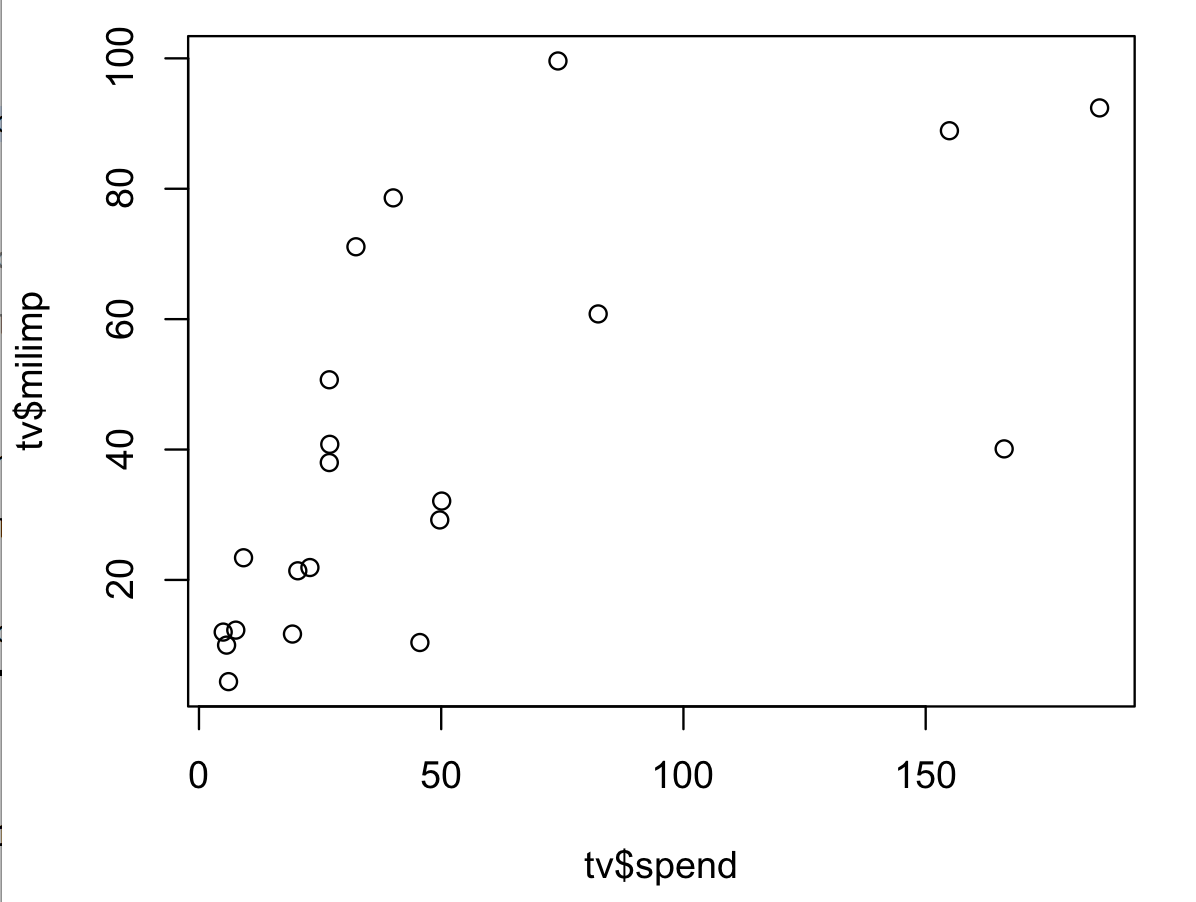
\includegraphics[width=.6\textwidth]{./notes/immagini/l9-fig1.png}
\end{figure}

La stima dei coefficienti viene fatta con

\begin{lstlisting}
n <- nrow(tv) // Numero di righe
beta2.hat <- cov(tv$spend, tv$milimp)/var(tv$spend) # Sarebbe beta_1
beta1.hat <- mean(tv$milimp) - beta2.hat * mean(tv$spend) # Sarebbe beta_0
\end{lstlisting}

e il modello ottenuto può essere visualizzato utilizzando (\texttt{abline} prende i coefficienti della retta da disegnare)

\begin{lstlisting}
plot(tv$spend, tv$milimp)
abline(beta1.hat, beta2.hat, lty = "dashed") # deve esserci il plot aperto perché compia la linea
\end{lstlisting}

\begin{figure}
	\centering
	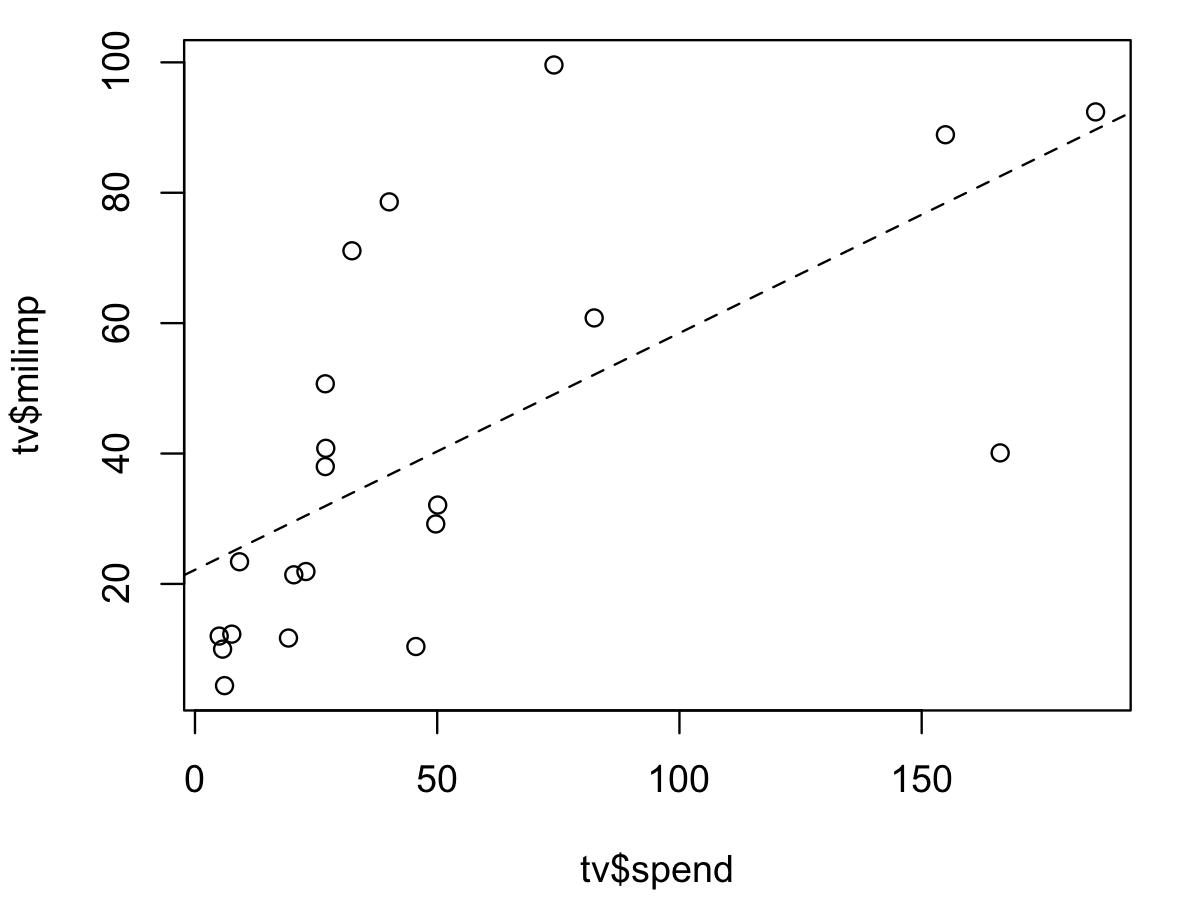
\includegraphics[width=.6\textwidth]{./notes/immagini/l9-fig2.png}
\end{figure}

\`{E} possibile calcolare e visualizzare i valori predetti con

\begin{lstlisting}
valori.predetti <- beta1.hat + beta2.hat * tv$spend # valori stimati
plot(tv$spend, tv$milimp)
abline(beta1.hat, beta2.hat, lty = "dashed")
points(tv$spend, valori.predetti, pch="X")
\end{lstlisting}

\begin{figure}
	\centering
	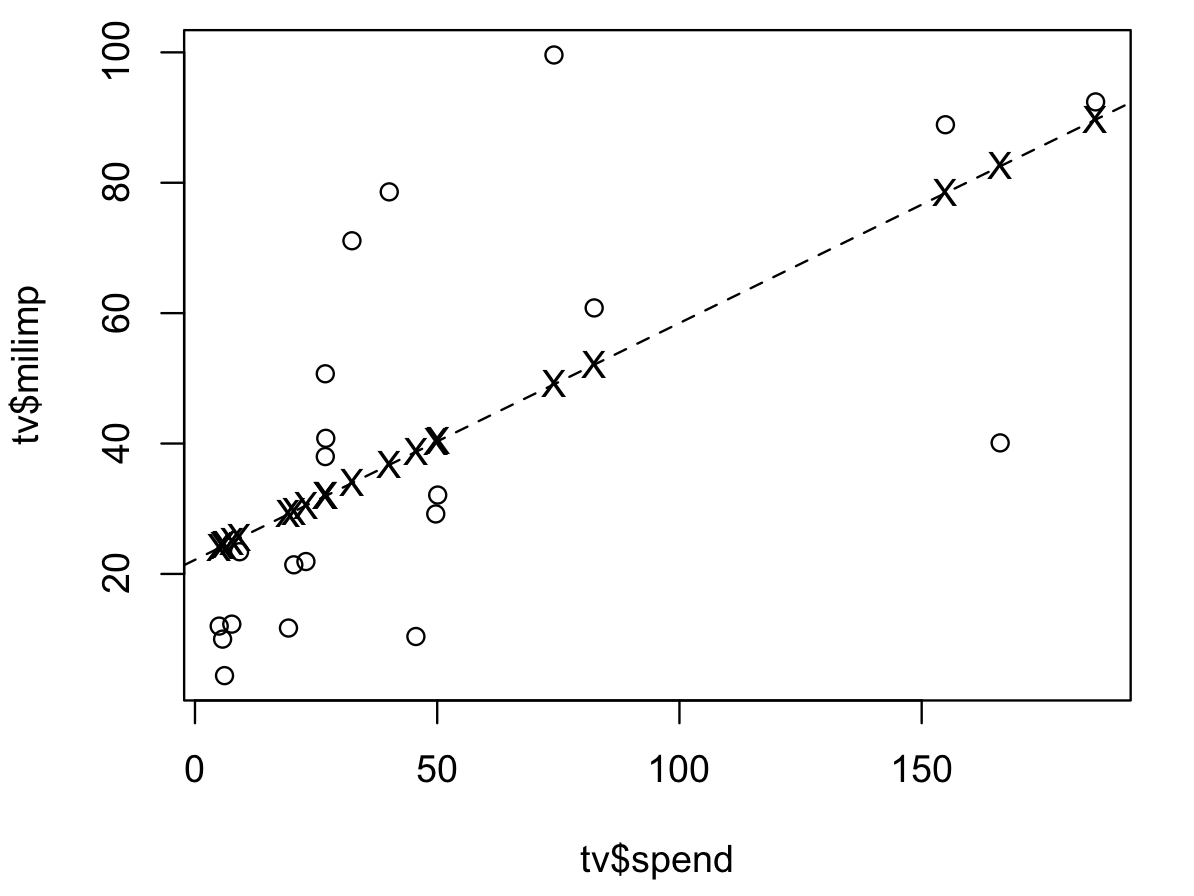
\includegraphics[width=.6\textwidth]{./notes/immagini/l9-fig3.png}
\end{figure}

Piccolo reminder: con \texttt{attach(tv)} si attacca il dataframe all'ambiente, in questo modo si può evitare di specificarlo quando è necessario accedere ai suoi campi dati.

Con i valori predetti è possibili calcolare i residui:
\begin{lstlisting}
residui <- milimp - valori.predetti
R2 <- 1 - var(residui)/var(milimp) # Otteniamo un R^2 del 42%

s2 <- sum(residui^2)/(n-2) # Varianza dei residui stimata
var.beta1.hat <- s2*(1/n + mean(spend)^2/sum((spend-mean(spend))^2))
var.beta2.hat <- s2/sum((spend-mean(spend))^2)
\end{lstlisting}

\subsubsection{Intervalli di confidenza}

Una volta stimate le varianze è possibile calcolare i gli intervalli di confidenza per i parametri del modello ottenuto. In questo caso si è fissato $ 1-\alpha = 95\% $

\begin{lstlisting}
# Estremi dell'intervallo di confidenza 1-alpha = 0.95 per beta1
beta1.lower <- beta1.hat - qt(0.975, df=n-2)*sqrt(var.beta1.hat)
beta1.upper <- beta1.hat + qt(0.975, df=n-2)*sqrt(var.beta1.hat)

# Estremi dell'intervallo di confidenza 1-alpha = 0.975 per beta2, ovvero il beta2 vero è dentro quell'intervallo con una probabilità del 95%
beta2.lower <- beta2.hat - qt(0.975, df=n-2)*sqrt(var.beta2.hat)
beta2.upper <- beta2.hat + qt(0.975, df=n-2)*sqrt(var.beta2.hat)

#Modo alternativo
beta2.IC <- beta2.hat + c(-1,1)*qt(0.975, df=n-2)*sqrt(var.beta2.hat) # ottiene i due valori
\end{lstlisting}

\subsubsection{Verifica d'ipotesi}

\begin{lstlisting}
# p-value
t2 <- beta2.hat / sqrt(var.beta2.hat) #t_oss per beta2
pvalue.t2 = 2*min(pt(t2,df=n-2), pt(t2, df=n-2, lower.tail=FALSE)) # Sceglie l'area più piccolo e la moltiplica x2.
# p-value = 0.001389084 -> per i dati a disposizione beta2.hat è significativo
\end{lstlisting}

\subsection{Il modello lineare di R}

\begin{lstlisting}
# Modello lineare calcolato da R
> m1 <- lm(milimp~spend, data=tv)
# descrizione del modello
> m1
# Console output:
# Call:
#	lm(formula = milimp ~ spend, data = tv)
#
# Coefficients:
# 	(Intercept)        spend  
# 	22.1627       0.3632  
summary(m1)

Call:
lm(formula = milimp ~ spend, data = tv)

Residuals:
Min      1Q  Median      3Q     Max 
-42.422 -12.623  -8.171   8.832  50.526 

Coefficients:
Estimate Std. Error t value Pr(>|t|)   
(Intercept) 22.16269    7.08948   3.126  0.00556 ** # Specifica la significatività secondo la scala sotto riportata
spend        0.36317    0.09712   3.739  0.00139 **
---
Signif. codes:  0 ‘***’ 0.001 ‘**’ 0.01 ‘*’ 0.05 ‘.’ 0.1 ‘ ’ 1

Residual standard error: 23.5 on 19  degrees of freedom # i gradi di libertà sono n-2 = 21-2
Multiple R-squared:  0.424, Adjusted R-squared:  0.3936 #Multiple R-squared = R2
F-statistic: 13.98 on 1 and 19 DF,  p-value: 0.001389 # i p-value sono sempre uguali

\end{lstlisting}

\begin{verbatim}
## Fare predizione con il modello di R
> p1 <- predict(m1) # predizione con gli stessi dati
> p1 <- predict(m1, newdata=dataframe) # con dati nuovi, su un dataframe con la stessa struttura

> p1 <- predict(m1, interval="prediction") # intervallo di previsione (c'è un warning che avvisa che si tratta per i valori futuri)

# Bande di confidenza con punti
# matplot fa il plot di una matrice
> matplot(sort(spend), p1[order(spend),], type="l", lty=c("solid","dashed","dashed"))
> points(spend, milimp, pch=16) #pch=16 -> pallino pieno

# .. inserire grafico ..

# Ma il modello non potrebbe essere migliore se fosse
## log(y) = c + k log(x)

> z <- log(milimp)
> x <- log(spend)
> m2 <- lm(z~x)
> summary(m2)

Call:
lm(formula = z ~ x)

Residuals:
     Min       1Q   Median       3Q      Max 
-1.30158 -0.23227  0.02061  0.38680  0.83035 

Coefficients:
            Estimate Std. Error t value Pr(>|t|)    
(Intercept)   1.2999     0.4236   3.069  0.00632 ** 
x             0.6135     0.1191   5.153 5.66e-05 ***
---
Signif. codes:  0 ‘***’ 0.001 ‘**’ 0.01 ‘*’ 0.05 ‘.’ 0.1 ‘ ’ 1

Residual standard error: 0.581 on 19 degrees of freedom
Multiple R-squared:  0.5829,    Adjusted R-squared:  0.561 
F-statistic: 26.55 on 1 and 19 DF,  p-value: 5.655e-05

> p2 <- predict(m2, interval="prediction")
> p2.originali = exp(p2) # ritorno alla scala originale

> matplot(sort(spend), p1[order(spend),], type="l", lty=c("solid","dashed","dashed"))
> points(spend, milimp, pch=16)
> lines(sort(spend), p2.originali[order(spend)], lty="solid", col=4) # linea per il nuovo modello

# .. inserire grafico ..

# Confronto dei due modelli

> residui.originali <- milimp - p2.originali
> var(residui.originali[,1]) # Varianza secondo modello
[1] 476.5299
> var(residuals(m1)) # varianza dei residui del primo modello
[1] 524.7054

# miglioramento (9%)
> ( var(residuals(m1)) - var(residui.originali[,1]))/var(residuals(m1))
[1] 0.09181452

####################################################
> cipolle <- read.table("lab-dati/cipolle.dat", header=TRUE, sep="\t")
> str(cipolle)
'data.frame':   84 obs. of  3 variables:
 $ dens: num  23.5 26.2 27.8 32.9 33.3 ...
 $ prod: num  223 234 222 222 197 ...
 $ loc : Factor w/ 2 levels "PL","V": 1 1 1 1 1 1 1 1 1 1 ...

# dens = piante al metro quadro
# prod = quantità prodotta
# loc  = località di produzione

> detach(tv)
> attach(cipolle)

# può essere utile guardare l'istogramma
> hist(dens) # istrogramma della densità
> hist(prod)
#ancora meglio è il boxplot
> boxplot(dens) # box plot
> boxplot(prod) # box plot
> plot(dens,prod) # diagramma di dispersione

# c'è una leggera curva, quindi conviene utilizzare la scala logaritmica per entrambe le variabili

> plot(log(dens), log(prod)) # i dati sono più lineare

## creazione dei modelli
> m1 <- lm(prod~dens)
> m2 <- lm(I(log(prod))~I(log(dens))) # I serve per applicare la trasformazione alle variabili

> summary(m1)

Call:
lm(formula = prod ~ dens)

Residuals:
    Min      1Q  Median      3Q     Max 
-53.507 -23.922  -1.372  12.149  95.296 

Coefficients:
             Estimate Std. Error t value Pr(>|t|)    
(Intercept) 196.53025    6.79309   28.93   <2e-16 ***
dens         -1.04775    0.08073  -12.98   <2e-16 ***
---
Signif. codes:  0 ‘***’ 0.001 ‘**’ 0.01 ‘*’ 0.05 ‘.’ 0.1 ‘ ’ 1

Residual standard error: 30.54 on 82 degrees of freedom
Multiple R-squared:  0.6726,    Adjusted R-squared:  0.6686 
F-statistic: 168.5 on 1 and 82 DF,  p-value: < 2.2e-16

> summary(m2)

Call:
lm(formula = I(log(prod)) ~ I(log(dens)))

Residuals:
     Min       1Q   Median       3Q      Max 
-0.53633 -0.14049  0.01342  0.15753  0.38104 

Coefficients:
             Estimate Std. Error t value Pr(>|t|)    
(Intercept)   7.74583    0.16227   47.73   <2e-16 ***
I(log(dens)) -0.73984    0.03885  -19.05   <2e-16 ***
---
Signif. codes:  0 ‘***’ 0.001 ‘**’ 0.01 ‘*’ 0.05 ‘.’ 0.1 ‘ ’ 1

Residual standard error: 0.2011 on 82 degrees of freedom
Multiple R-squared:  0.8156,    Adjusted R-squared:  0.8134 
F-statistic: 362.7 on 1 and 82 DF,  p-value: < 2.2e-16

# Confronto grafico tra i due modelli

> p1 <- predict(m1)
> p2 <- predict(m2)

> plot(log(dens), log(prod)) # retta in scala logaritmica
> lines(log(dens), p2)

> plot(dens,prod) # plot in scala originale
> lines(dens[order(p2)], exp(sort(p2)))

> plot(dens,prod) ## entrambe le rette
> lines(dens[order(p2)], exp(sort(p2)))
> abline(m1) 

# analisi grafica di un modello
> plot(m1) # mostra una serie di grafici tra cui quello dei residui
> plot(m2) # da un errore strano (poco male)


\end{verbatim}